\documentclass[a4paper]{article}
\usepackage{url}
\usepackage{multirow}
\usepackage{INTERSPEECH2021}
\usepackage{cite}
\usepackage{tablefootnote}
\usepackage{color}
\usepackage{booktabs}
\usepackage{graphicx} 
\usepackage{epstopdf, multirow}
\usepackage{pifont}
\usepackage{footnote}
\usepackage{soul}
\usepackage{amssymb}% http://ctan.org/pkg/amssymb
\usepackage{pifont}%http://ctan.org/pkg/pifont
% \usepackage{biblatex}
% \renewcommand*{\bibfont}{\footnotesize}
\newcommand{\cmark}{\ding{51}}%
\newcommand{\xmark}{\ding{55}}%
% \usepackage{comment}
\newcommand{\textoverline}[1]{$\overline{\mbox{#1}}$}
\usepackage{todonotes}
\setlength{\marginparwidth}{45pt}
\setlength{\intextsep}{1pt plus 0pt minus 3pt} %distance between floats on the top or the bottom and the text
\setlength{\textfloatsep}{1pt plus 0pt minus 4pt}%distance between two floats
\setlength{\floatsep}{1pt plus 0pt minus 2pt}%distance
\title{Unsupervised Acoustic Unit Discovery by Leveraging a Language-Independent Subword Discriminative Feature Representation}

% \title{Learning a Language-independent Subword Discriminative Feature Representation for Unsupervised Acoustic Unit Discovery}
\name{Siyuan Feng$^{1}$,
Piotr \.Zelasko$^{2,3}$, 
Laureano Moro{-}Vel{\'{a}}zquez$^{2}$ and
Odette Scharenborg$^1$
\thanks{Code: \texttt{https://github.com/syfengcuhk/mboshi}. We thank Lucas Ondel for valuable discussion on the evaluation software.}
}

%The maximum number of authors in the author list is twenty. If the number of contributing authors is more than twenty, they should be listed in a footnote or in acknowledgement section, as appropriate.
\address{
  $^{1}$Multimedia Computing Group, 
  Delft University of Technology, Delft,  the Netherlands
  $^{2}$Center for Language and Speech Processing, $^{3}$Human Language Technology Center of Excellence, \\Johns Hopkins University, Baltimore, MD, USA
  }% \\
 %$^2$Department of Electronic Engineering, The Chinese University of Hong Kong, Hong Kong}
\email{\{S.Feng, O.E.Scharenborg\}@tudelft.nl, \{petezor,laureano\}@jhu.edu}

\begin{document}

\maketitle
% 
\begin{abstract}
% \todo[]{212 words, exceeding 200-word limit}
This paper tackles  automatically discovering  phone-like acoustic units (AUD) from unlabeled speech data. 
Past studies usually proposed single-step approaches.
We propose a two-stage approach: the first stage learns a subword-discriminative feature representation, and the second stage applies clustering to the learned representation and obtains phone-like clusters as the discovered acoustic units. In the first stage, a recently proposed  method in the task of unsupervised subword modeling is improved by replacing a monolingual out-of-domain (OOD) ASR system with a multilingual one to create a  subword-discriminative representation that is more language-independent. In the second stage, segment-level k-means is adopted, and two methods to represent the variable-length speech segments as fixed-dimension feature vectors are compared. Experiments on a very low-resource Mboshi language corpus   show that our approach outperforms state-of-the-art AUD in both normalized mutual information (NMI) and F-score. The multilingual ASR improved upon the monolingual ASR in providing OOD phone labels and in estimating the phone boundaries. 
A comparison of our systems with and without knowing the ground-truth phone boundaries showed a 16\% NMI performance gap, suggesting that 
the current approach can significantly benefit from improved phone boundary estimation.
% one direction to improve our approach concerns improving phone boundary estimation.
% future research should focus on improving  phone boundary estimation. 
 \end{abstract}
\noindent\textbf{Index Terms}:  
Acoustic unit discovery, unsupervised subword modeling, zero-resource

\section{Introduction}
% Recent advancements on automatic speech recognition (ASR) can be attributed to two main factors: successful application of deep neural networks (DNNs) and large amounts of  annotated speech data for model training. Nevertheless, t
There are around $7,000$ spoken languages in the world \cite{austin2011cambridge}, most of which lack transcribed speech data \cite{adda2016breaking}. Conventional supervised acoustic modeling strategies \cite{dahl2011context,chan2016listen} therefore cannot be applied directly to build ASR systems for such low-resource languages. As a result, current high-performance ASR schemes are available only for a very small number of languages \cite{feng2021how}.
To facilitate ASR for low-resource languages,  unsupervised acoustic modeling  has been gaining research interest  recently \cite{lee2012a,I3EWang,chen2015parallel}.  Unsupervised acoustic modeling aims to discover basic speech units that represent  all the sounds in a target language by making a  \textit{zero-resource} assumption  \cite{dunbar2017zero}, i.e., for a target language, only speech recordings are available while transcriptions and phoneme inventory (or its size) information are unknown. 

There are two mainstream research strands in unsupervised acoustic modeling. The first strand, \textit{acoustic unit discovery (AUD)} \cite{ondel2016variational,lee2012a}, formulates the problem as discovering a finite set of phone-like acoustic units \cite{lee2012a,I3EWang,Ondel2019Bayesian}. 
% Studies on the AUD task can be traced back to early 2010s \cite{lee2012a,Wang2013unsup_mining}. 
The second strand, \textit{unsupervised subword modeling (USM)} \cite{dunbar2017zero,Dunbar2019}, formulates the problem as learning a frame-level feature representation  that can distinguish subword units (phonemes)  and is robust to speaker variation \cite{chen2015parallel,oord2017neural,heck2017feature}. 
Studies on the USM task were mostly driven by the 
% Zero Resource Speech Challenges (ZeroSpeech) 
ZeroSpeech Challenges
\cite{dunbar2017zero,Dunbar2019,Dunbar2020zero}. 
In essence, the USM task can be considered as learning an intermediate representation towards achieving the goal of AUD \cite{Feng2019combining}. 

This study addresses the AUD task. 
Two main types of approaches to  the AUD task were investigated in the past. The first type adopts  self-supervised  learning algorithms and uses a quantization layer to obtain a finite set of discovered acoustic units \cite{oord2017neural,baevski2020vqwav2vec,Niekerk2020vector}. The second type adopts Bayesian non-parametric versions of the hidden Markov model (HMM) \cite{lee2012a,Ondel2019Bayesian,Yusuf2020hierarchical}. The combination of self-supervised learning and Bayesian approaches was also studied \cite{Ebbers2017,ondel2018bayesian}.
All the studies mentioned above proposed single-step approaches. In contrast, the present study proposes a two-stage learning framework: the first stage learns a frame-level subword-discriminative  feature representation  (i.e., the USM task); the second stage  applies clustering techniques to the  learned frame representation to obtain a set of clusters as the discovered acoustic units. 
% The advantage of the first stage is that,
% My suggestion:
% Some studies suggest that, s
Subword-discriminative feature representations can provide a better separation between sounds than spectral features: In a subword-discriminative representation,  two   examples of the same phoneme are closer while those of different phonemes are further apart than in an  MFCC representation. This is a    highly desired property in     clustering-based acoustic unit discovery \cite{I3EWang,Bhati2019unsupervised}, which motivates us to propose a two-stage learning framework.

% %Instead of the paragraph:
% Comparing to spectral   representations e.g. MFCC,  in a subword-discriminative feature representation, speech of the same phoneme is closer while speech of different phonemes is further apart \cite{dunbar2017zero}. 

% This is a highly desired property in     clustering-based phoneme-like unit discovery \cite{I3EWang,Bhati2019unsupervised}, which motivates us to  propose such a two-stage learning framework.

Specifically, in the first stage of the framework proposed in this study, we leveraged and improved a USM approach from a previous study \cite{feng2020unsupervised}. This approach trains an autoregressive predictive coding (APC)  model \cite{Chung2019} followed by a cross-lingual DNN model to  extract bottleneck features  (BNFs)  as the   subword-discriminative representation. 
Previous results  \cite{feng2020unsupervised,feng2020effectiveness} employing a \textit{single} out-of-domain (OOD) language's resources to generate OOD phone labels for cross-lingual DNN training,  provided state-of-the-art performance in USM tasks. 
Here, we aim to improve this approach further and, for the first time, use it for a different task: AUD. 
To leverage an OOD ASR system to generate OOD phone labels, We propose to use \textit{multiple} OOD languages' resources to build a more language-independent OOD ASR system than in our previous work \cite{feng2020unsupervised}. 
%We propose the use of \textit{multiple} OOD languages' resources to build a more language-independent OOD ASR system than in our previous work \cite{feng2020unsupervised} to  provide the OOD phone labels for benefiting target  language acoustic modeling. 
Because different languages have different phoneme inventories, we hypothesize that OOD phone labels that capture a more extensive set of sounds will be more useful for acoustic modeling of a target language. We will compare the use of multiple versus a single OOD language resources in this paper.
% My recommendation to add after the citation: ... \cite{feng2020unsupervised}. Our hypothesis is that an acoustic model that considers a larger variety of sounds will be more useful for target language representation.
% modeling the target unknown language.
% To our knowledge the  approach in \cite{feng2020unsupervised} has not been studied for the AUD task.
% on ZeroSpeech 2017 \cite{dunbar2017zero} as well as Libri-light \cite{kahn2019librilight} databases. 
In the second stage of our framework,  the $k$-means algorithm is adopted for speech segment clustering. To that end, first, phone segment boundaries are estimated using an OOD ASR via decoding \cite{feng2016exploit}. The resulting variable-length segments need to be represented as fixed-dimension vectors, 
% A key issue in segment clustering is to represent arbitrary-length segments as fixed-dimension vectors \cite{levin2013fixed}. 
for which we compare two often adopted approaches \cite{kamper2017embeded,Bhati2019unsupervised,feng2016exploit}: an average-based method \cite{I3EWang} and a downsampling method \cite{levin2013fixed}.  
We measure the sensitivity of our AUD approach's performance to   the number of discovered acoustic units,
% We   measure the proposed approach's AUD performance sensitivity to the number of discovered acoustic units,
because the phone inventory size of a target language is usually unknown. 
% While the latter method was more recommended by recent works, we do not find its superiority. 
% Both methods outperform a frame-level clustering baseline.  
The experiments   are carried out   on a very low-resource language, Mboshi  \cite{Godard2018mboshi} ($4.5$ hours of unlabeled speech).

% demonstrate that our   system outperforms   state of the art in the AUD task \cite{Yusuf2020hierarchical,Ondel2019Bayesian}.
% , and the advantage of applying a language-independent OOD ASR is mainly on improving the phonetic relevance of the discovered units, rather than on improving phone boundary estimation.
% It is expected that  subword-discriminative feature representations are highly desired for  feature clustering in the AUD task \cite{feng2016exploit}

% \section{Related works}
% \label{sec:related_works}
% There are two main types of approaches to  the AUD task. The first type adopts  self-supervised representation learning algorithms and applies a quantization layer to obtain a finite set of discovered acoustic units \cite{oord2017neural,baevski2020vqwav2vec,Niekerk2020vector}. The second type adopts Bayesian non-parametric versions of the hidden Markov model (HMM) \cite{lee2012a,Ondel2019Bayesian,Yusuf2020hierarchical}. The combination of self-supervised learning and Bayesian approaches was also studied \cite{Ebbers2017,Glarner2018Full,ondel2018bayesian}.




\section{Proposed two-stage approach}
% The two stages of our proposed approach to the AUD task are described 
% Our  proposed approach to the AUD task consists of two stages. The first stage learns a subword-discriminative feature representation. The second stage applies $k$-means algorithm to cluster target speech based on the learned feature representation and obtain a finite set of phoneme-like acoustic units. The two stages are described 
% in Sections \ref{subsec:approach_1st} and \ref{subsec:approach_2nd_stage} respectively.
\subsection{Stage 1: subword-discriminative feature learning}
\label{subsec:approach_1st}
The goal of this stage is to learn a frame-level subword-discriminative feature representation.
% feature representation that can distinguish subword units of a target language and is robust to speaker variation. 
%The approach in  is adopted, modified and improved in this paper.
% with modifications and improvements. 
The  general framework of the first stage of our proposed approach, based on \cite{feng2020unsupervised}, consists of an 1) APC model, which creates the APC features that are used as input to a  2) DNN acoustic model (AM) together with the frame-level phone labels obtained from 3) an OOD (non-target language)  ASR system
(see Figure \ref{fig:framework_1st}). After training the DNN AM, BNFs are extracted from the bottleneck layer of the DNN as the desired subword-discriminative representation.

\begin{figure}[!t]
    \centering
    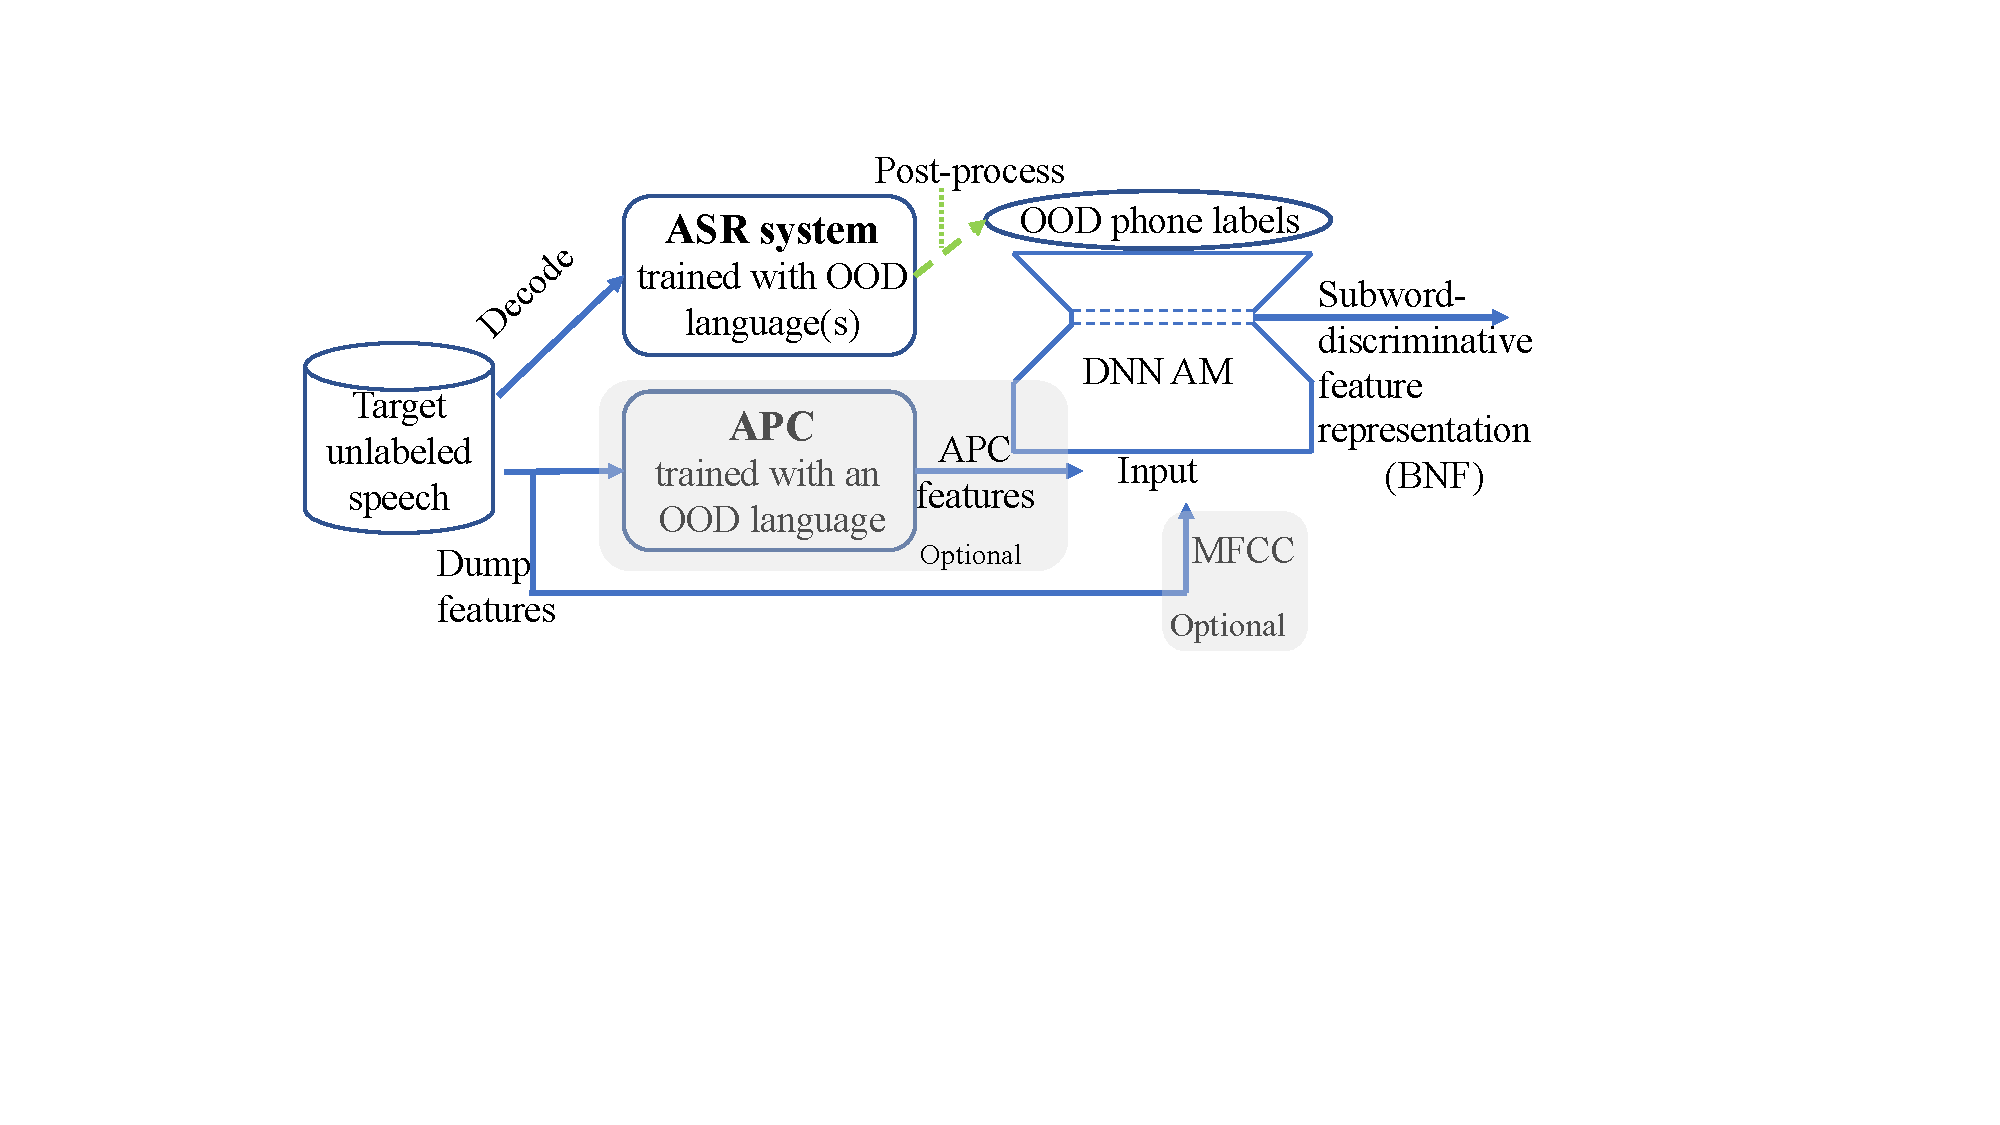
\includegraphics[width =  \linewidth]{LaTeX/USM.pdf}
    \caption{The first stage in the proposed approach. ``OOD'' denotes out-of-domain, i.e. non-target language(s). The input to the DNN AM is either APC features or MFCCs but not both.}
    \label{fig:framework_1st}
\end{figure}
%It mainly consists of   

APC is a self-supervised learning model without the need of transcriptions for training. It is trained to predict a future speech frame $n$ steps ahead (named \textit{prediction step}) based on the current and past frames of an utterance \cite{Chung2019}. APC is incorporated in \cite{feng2020unsupervised} to extract \textit{APC features} as input to the DNN AM (see Figure \ref{fig:framework_1st}), owing to its ability to make phonetic and speaker information   in speech   more separable than  MFCC.  
% My suggestion for the next paragraph:
In this study we tackle an extremely low-resource scenario ($4.5$ h), however
% evaluate if APC models can provide effective representations in an extremely low-resource scenario ($4.5$ hours). 
our previous work \cite{feng2020unsupervised} suggests that a larger training dataset (more than $50$ h) is needed to obtain effective APC features, thus we opt  for using an APC model trained with a well-resourced OOD language. Note that a recent study \cite{riviere2020unsupervised} found that self-supervised models trained on one language can be used to represent another language with certain success. In our experiments we compare (1)  APC features extracted by an APC model which is trained with an OOD language; and (2) MFCC features (hence bypassing the APC model); as the input  to the DNN AM (see Figure \ref{fig:framework_1st}). 

% \cite{feng2020unsupervised} indicated that the   APC model only showed noticeable effectiveness when more than $50$ hours of target language   data was used for training. As the current study assumes  an extremely low-resource scenario ($4.5$ hours), it is unknown whether APC is still effective. 
% % However the present study assumes  an extremely low-resource scenario with only $4.5$ hours of target (Mboshi) speech.  It remains unknown whether APC is effective with this scenario. 
% \todo{Odette's original comments are   below:}
% A recent study \cite{riviere2020unsupervised} found that self-supervised models trained on one language can be used to represent another language with certain success. This  inspired us to compare (1)  using an APC model trained with an OOD language's speech; and (2) bypassing the APC model and feeding MFCC  to the DNN AM (see Figure \ref{fig:framework_1st}). 
% In other words, either the APC features or MFCC features are fed as input to the DNN AM (see Figure \ref{fig:framework_1st}).
% \subsubsection{s}

The  DNN AM in Figure \ref{fig:framework_1st}
% contains a bottleneck layer in the middle.
% Bottleneck features (BNFs)  extracted from a BN layer of a DNN AM are known to carry phonetic information while being largely speaker-independent \cite{vesely2012language_independent}. 
is trained with target language acoustic data. %, using APC features or MFCCs as input features.
% APC features (or MFCCs) of the target unlabeled speech data. 
Frame-level phone labels required for training the DNN AM are obtained using an OOD (non-target)  ASR system  \cite{feng2020unsupervised}: a  target speech utterance is decoded by the OOD ASR system so that every frame is assigned  a  phone label generated by the OOD ASR. 
By this means, an OOD language's phonetic knowledge is exploited for the target language acoustic modeling.
% the OOD phone labels provide phonetic representation for the target speech from a cross-lingual perspective. 
BNFs are then extracted from the bottleneck layer of the trained DNN as the desired subword-discriminative representation.
% As phoneme inventories  of an OOD language may not completely cover all 

%One limitation of the OOD     phone labeling   is that speech sounds that occur in the target language but not in the OOD language are not well represented by the OOD phone labels. To  overcome this, we propose to % exploiting multiple OOD languages' resources to 

The language-independent OOD ASR system leverages multiple phonetically diverse languages' resources. We use International Phone Alphabet (IPA) symbols \cite{international1999handbook}   to represent the phonemes of the different OOD languages, thus creating a phoneme inventory of the multilingual ASR system that is more language-independent \cite{zelasko2020sounds} than that of a monolingual OOD. This also enables acoustic information sharing of  the
% same  or  very close\footnote{We realise that sounds from two languages with the same IPA symbol may not be entirely the same but for the purpose of this task we do treat them as the same phoneme.}  
same or similar 
sounds from multiple  languages during   ASR  training.   A multilingual ASR system captures a wider phonetic space and has more different phone labels than a monolingual ASR system, thus is expected to provide more refined OOD phone labels for the target speech than a monolingual  ASR system. %We compare the use of multilingual versus monolingual OOD ASR systems to generate OOD phone labels for target speech to train DNN AMs and extract BNFs.
% Using the multilingual OOD ASR system to assign IPA phone labels to target speech frames, we will show it provides better phone labels than a monolingual OOD ASR system, which is essential for the AUD task.
% , frames of target speech are assigned with IPA phone labels.  We will show the multilingual OOD ASR system provides better phone labels  for the target speech  than a monolingual OOD ASR system. 

Another modification to the approach in \cite{feng2020unsupervised} is adding a post-processing step to  the OOD ASR based phone labels (see Figure \ref{fig:framework_1st}). Essentially, the post-processing aims to refine the phone labels from an OOD ASR via re-aligning:
% re-aligns  the  phone labels from an OOD ASR: 
First, we train an HMM with the OOD phone labels and Mboshi acoustic data; second, we generate the HMM phone alignments as the  desired frame-level label supervision (rather than the output of an OOD ASR) to train the DNN AM. We  experimentally found that the post-processing step  consistently improves the AUD performance. Presumably, it refines the OOD phone labels by leveraging contextual information in the Mboshi acoustic data.

% we experimentally found that  via training an HMM with the OOD phone labels and Mboshi acoustic data, followed by 
% % the OOD phone labels and Mboshi speech are used to train a GMM-HMM, followed by
% using the HMM phone alignments as supervision to train the DNN AM (instead of directly using OOD phone labels   as DNN supervision \cite{feng2020unsupervised}), the AUD performance is improved. %This post-processing step is .
%Hence this post-processing method is applied throughout this paper.

% , comparing to directly use the OOD phone labels in DNN AM training. 

% As was done in \cite{feng2020unsupervised}, While phone labels generated by an OOD ASR system can be directly taken as supervision to train the DNN AM, 
% We found  improved by first training a GMM-HMM  with Mboshi speech and the OOD phone labels, followed by using the forced-aligned phone labels as supervision for DNN AM training. We adopted the latter method throughout this paper.    
% , and (2) an APC model trained  with an out-of-domain (OOD)  language is effective. In this study we will compare  


% Figure \ref{fig:framework_1st}.
% \todo[inline]{
%   Concise description of IS2020 approach\\
%      emphasize we're using universal IPA phone symbols to train an OOD (multilingual) ASR system.\\
     
%  }

\subsection{Stage 2: speech segment representation and clustering}
\label{subsec:approach_2nd_stage}
This stage applies $k$-means clustering to the subword-discriminative feature representation learned by the first stage to obtain a finite set of clusters, each of which resembles a phone-like acoustic unit. The discovered units are the outcome of the proposed two-stage approach.  

Speech clustering can be realized at the segment level \cite{LeeSoongJuang} or at the frame level   \cite{chen2015parallel}.  
% Segment-level speech clustering   \cite{Bhati2019unsupervised,levin2013fixed} treats each variable-length speech segment as one sample during clustering.
For segment-level clustering, we need the phone segment boundaries, and the segments need to be  represented as fixed-dimension vectors. In order to obtain the segment boundaries,  we rely on the OOD ASR system (see Section \ref{subsec:approach_1st}):  after decoding the  target speech data, phone boundary information is obtained by finding discontinuities of the frame-level OOD phone labels. This phone boundary estimation method is similar to \cite{feng2016exploit}, except that here we are using a multilingual and  IPA symbol-based OOD ASR system.

This study compares two methods to obtain the fixed-dimensional segment representation. The first is a \textbf{downsampling}   method \cite{levin2013fixed} as suggested by \cite{kamper2017embeded,Bhati2019unsupervised}: a variable-length speech segment is cut into a fixed number ($s$) of consecutive sub-segments, and 
the averages over $d$-dimensional frame-level feature vectors within each sub-segment are concatenated 
% within each sub-segment its average over all frame-level feature vectors ($d$-dimension) is calculated,  concatenated 
to form a  feature vector of dimension $s \times d$ for each segment.
Note that when $s=1$, the method is equivalent to an \textbf{average}-based method \cite{I3EWang} which takes the average of the frame-level features over all the frames in a segment. The downsampling method with a large $s$ captures abundant temporal information which is not captured by the average method, however a large $s$ leads to a high dimension of the segment-level feature vector which might adversely affect $k$-means. 
%given a speech segment of an arbitrary $t$,  $\{\bm{x_1}, \ldots, \bm{x_t}\}$

% \todo[inline]{Frame-level clustering and pros/cons, state we will compare our segment-level clustering against frame-level one}
% To compare against segment-level clustering, we   
Segment-level clustering with the two methods mentioned above are compared with a frame-level clustering system as a baseline, which applies  $k$-means (same as  in the proposed systems)
% same  $k$-means algorithm as the proposed systems 
to a frame-level feature representation. While circumventing the need for segment boundaries and the need for fixed-length segment representations, frame-level clustering  tends to produce over-fragmented discovered units \cite{wu2018optimizing,feng2019_TASLP}.  
Finally, we report an ``upperbound'' segment-level system by assuming the availability of golden phone  boundary information while keeping the other settings unchanged. This allows us to quantify the performance degradation attributed to imperfect  phone boundary estimation.
%We experimentally validate this and compare against segment-level clustering.

%  \todo[inline]{  leave the investigation of alternative clustering algorithms in this task for future study}
  %Aliquam quis orci consectetur nulla luctus ullamcorper. Suspendisse finibus luctus erat a dapibus.

\section{Experimental setup}
\label{sec:setup}
\subsection{Evaluation metrics}
\label{subsec:setup_eval}
% To compare with  past studies, 
% make performance comparable to past studies, 
We use two common metrics in the AUD task \cite{ondel2016variational,Ebbers2017,Yusuf2020hierarchical} to compare with past studies: 
% Following recent past studies \cite{ondel2016variational,ondel2017bayesian,Ondel2019Bayesian,Yusuf2020hierarchical}, the AUD performance is evaluated by two metrics from two perspectives. 
normalized mutual information (\textbf{NMI})  and \textbf{F-score}. NMI   measures the statistical dependency between discovered units (DUs) and ground-truth phone units (GUs), which is computed based on a frame-level confusion matrix of DU and GU  (see \cite{Yusuf2020hierarchical} for details). An NMI value ranges between $0$  and $100\%$, with a higher value  indicating a higher consistency between DUs and GUs, hence is preferred. F-score is  the harmonic mean of recall (R) and precision (P). It is used to measure  the accuracy of the phone segmentation. 
A tolerance of $\pm20$ ms is set when computing F-score values. 
Higher F-score, R and P   are preferred. %Both NMI and F-score are calculated based on  

\subsection{Databases}


\label{subsec:setup_database}
The AUD  performance    is evaluated on a corpus
 containing $5,130$ sentences spoken by three speakers of the Mboshi language  \cite{Godard2018mboshi}, 
for a total amount of $4.5$ hours. Automatically generated Mboshi phone alignments are available, but are not used during   system development. Note that the DNN AM in our system is trained and evaluated on the entire Mboshi dataset without training-test partition, as we are tackling an unsupervised learning problem. This  is also consistent with  the  studies   \cite{Yusuf2020hierarchical,Ondel2019Bayesian}.

Speech from $13$ phonetically diverse languages \cite{zelasko2020sounds} is used to train the OOD multi-/monolingual ASR systems. $5$ languages are from GlobalPhone  \cite{schultz2002globalphone}: Czech ($24$ h), French ($23$ h), Spanish ($12$ h), Mandarin ($15$ h) and Thai ($23$ h). The other $8$ languages are from IARPA Babel: Cantonese ($127$ h), Bengali ($55$ h), Vietnamese ($78$ h), Lao ($59$ h), Zulu ($54$ h), Amharic ($39$ h), Javanese ($41$ h) and Georgian ($45$ h).

% For systems incorporating an APC model in the first stage, the data that is used to train the APC model is taken from the \textit{unlab-600} set ($600$ hours) of Libri-light (English) \cite{kahn2019librilight}.

% \todo[inline]{Mboshi, 5 GlobalPhone languages and 8 Babel languages. Libri-light unlab-600 (apc when applicable)}
 
% \todo[inline]{NMI, F-score}

\subsection{Implementation of stage 1}
\label{subsec:setup_stage1}
The APC model included in the first stage of the proposed model is taken from our previous study \cite{feng2020unsupervised}: 
it has $5$ LSTM layers of dimension $100$ with residual connections. The prediction step is $5$. %[to win space]The input features to the APC model are  MFCCs with cepstral mean normalization (CMN). 
The model was trained with the Libri-light (English) \textit{unlab-600 (hour)} set \cite{kahn2019librilight}.
APC features are extracted from the top layer of the APC model.
% The output from the top layer of the APC model is extracted as the APC features.% for the Mboshi speech.

% The APC model is trained by  following  implementation  in \cite{feng2020unsupervised}: the model has $5$ LSTM layers of dimension $100$ with residual connections. The prediction step is $5$. The input features to the APC model are  MFCCs with cepstral mean normalization (CMN). 
% % The model is trained for $100$ epochs. 
% After training, output from the top layer of the APC model is extracted as the APC features.

We developed $2$ multilingual systems and $5$ monolingual systems, differing  only in the training   languages: \textbf{Multi-5} denotes the multilingual system trained with the 5 GlobalPhone languages; \textbf{Multi-13} denotes the multilingual system trained with all 13 GlobalPhone+Babel languages; \textbf{Mono-CZ, Mono-FR, Mono-SP, Mono-MA, Mono-TH} are five monolingual systems, each trained with one GlobalPhone language, i.e., Czech, French, Spanish, Mandarin, and Thai, respectively.
We do not report any monolingual system trained on each of the Babel languages because of its inferior AUD performance -- possibly explained by the large recording condition mismatch  between the Babel languages and Mboshi.
IPA symbols are used to represent the basic acoustic units, and the mapping from  orthographic transcriptions  to IPA symbol sequences is obtained by LanguageNet G2P models \cite{hasegawa2020grapheme}.

The multilingual and monolingual OOD ASR systems are trained using Kaldi \cite{povey2011kaldi}, adopting a hybrid  architecture \cite{dahl2011context}, following implementation   in \cite{feng2021how}. The AM adopts a factorized time-delay neural network (TDNNF) consisting of $12$ layers with a hidden dimension of $1024$
% and bottleneck dimension of $128$ 
and Resnet-style skip connections, trained with the LF-MMI criterion \cite{povey2016purely} for $4$ epochs, with a starting learning rate (LR) of $10^{-3}$. The input features consist of $43$-dimension high-resolution MFCC+pitch features and $100$-dimension i-vectors. The language model (LM) is a uni-gram phonotactic LM instead of an RNNLM, as we intend the OOD ASR phone labeling process to be  minimally affected by the OOD language phonotactics. The LM is trained with the training data transcripts using SRILM \cite{Stolcke02srilm--}.

% phone labels for target speech generated by an OOD ASR system   mainly reflect acoustic properties rather than OOD language phonotactics. 

% are used to convert orthographic transcriptions in GlobalPhone and Babel corpora into IPA symbol sequences in order to train the ASR  systems. 
The DNN AM for Mboshi is trained using either APC features or MFCC features of the Mboshi data. 
For each of  the $7$ multi/monolingual OOD ASR systems, the generated and post-processed (see Section \ref{subsec:approach_1st}) OOD phone labels are used    to train one DNN AM with MFCC as input features, resulting in $7$ DNN AMs. 
For the sake of simplicity, to test the effectiveness of the APC features,  only for the system employing \textbf{Multi-13} (the best-performing OOD ASR),  an additional DNN AM is trained with APC features instead of MFCCs. 
% We additionally implement one DNN AM using APC features as input features and \textbf{Multi-13} based OOD phone labels, in order to test the effectiveness of APC in the AUD task.
%My suggestion (as in the comment):
%All the ASRs (mono and multilingual) are employed to train a DNN-AM using MFCCs as input features. For the sake of simplicity, only the ASR providing the best results in the previous stage will be used in combination with APC features to train and evaluate another DNN-AM.
The Mboshi DNN AM adopts a  TDNNF structure similar to that of the OOD ASR AM, except: a $40$-dimension bottleneck layer is  placed below the top TDNNF layer; i-vector input is not included as we found it deteriorated the performance in our preliminary results (not included in this paper);
% , not included in this paper for the sake or simplicity; 
the model is trained for $20$ epochs with a smaller LR of $2.5\cdot 10^{-4}$ to stabilize the training procedure due to only $4.5$ hours of training material\footnote{Speed perturbation based data augmentation techniques were tried but no improvement was found, thus are not applied.}.  After training the  DNN AM, the BNF for the Mboshi representations are extracted from the bottleneck layer  as the  learned frame-level subword-discriminative representation, and are used as input to the 
% to carry out clustering in the 
second stage of the proposed system.
% \begin{itemize} 
%     \item Multi-5: multilingual OOD ASR system trained with 5 GlobalPhone languages.
%     \item Multi-13: multilingual OOD ASR system trained with 5 GlobalPhone plus 8 Babel languages.
%     \item Mono-CZ, Mono-FR, Mono-SP, Mono-MA, Mono-TH: five monolingual OOD ASR systems, each trained with a GlobalPhone language as indicated in their names.
% \end{itemize}

% \begin{table}[!t]
% % \renewcommand\arraystretch{0.4}
% \centering
% \caption{S.}
% % \resizebox{ 0.9 \linewidth}{!}{%
% \begin{tabular}{l|c|c|cccc}      
% % \hline      
% \toprule
% d\\
% \bottomrule
% \end{tabular}%
% % \footnotetext{`speakers-R/-L' denotes speakers with rich/limited speech data}
% % }
% \label{tab:setup_ood_asr_setting}
% \end{table}


% \todo[inline]{OOD ASR system, DNN AM}

\subsection{Implementation of stage 2}
\label{subsec:setup_stage2}

The $k$-means algorithm is implemented using \cite{scikit-learn}. 
Unless specified differently, the number of clusters is empirically set to $50$.
% For each segment-level or frame-level clustering, we repeat clustering $5$ times using different  random initialization and report the means and standard deviation of NMI and F-score. 
Segment-level clustering is done on all the learned subword-discriminative representations of the different DNN AMs  (i.e., 1 for each OOD system). 
For segment-level clustering, the speech segment boundaries are estimated using the OOD ASR system in the first stage. 
The downsampling method with $s$ in $\{2,3,4,5\}$ and the average based method are compared for obtaining the fixed-dimension segment  representation. 
The frame-level clustering baseline and the upperbound segment-level system are based on the feature representation  learned using \textbf{Multi-13}. Since the optimal setting of the number of clusters is unknown, we tested a range between $30$ and $70$. 
% This allows us to measure the proposed approach's AUD performance sensitivity to the number of discovered units.
% bet of  segment-level clustering 


% is   implemented, based on the subword-discriminative feature representation  learned using the \textbf{Multi-13} ASR system in the first stage. An ``upperbound'' system 

% is reported by leveraging the golden phone segmentation boundary information, also . %While the upperbound  is \textit{not} an unsupervised AUD system, it  measures the performance gap attributed from imperfect phone segmentation boundary estimation. 
%the best AUD performance our subword-discriminative representation could achieve

 
% \todo[inline]{segment vs frame, num of clusters, upperbound system which makes use of golden phone segment boundary information}

\section{Results and discussion}
\label{sec:results}
For each experiment, we repeat $k$-means clustering $5$ times with different  random initialization and report NMI and F-score  in means $\pm$ standard deviation.

\subsection{Evaluation of stage 1: Effect of frame-level subword-discriminative feature representations}
\label{subsec:multi_mono_asr}
\begin{table}[!t]
\renewcommand\arraystretch{0.4}
\centering
% \caption{Results of the multi-/monolingual OOD ASR systems and SotA.} 
\caption{Comparison of adopting a multi-/monolingual OOD ASR system  in stage 1 of our approach  and SotA \cite{Ondel2019Bayesian,Yusuf2020hierarchical}.}
% ``\cmark/\xmark'' denotes a system   using APC/MFCC features as input features.  }
\resizebox{ 0.83 \linewidth}{!}{%
\begin{tabular}{clcc}      
% \hline      
\toprule
Input &   system & NMI ($\%$) & F-score ($\%$)\\
\midrule
\multirow{7}{*}{MFCC}
& Mono-CZ&$40.87\pm0.14$ &$63.01\pm0.06$\\
& Mono-FR&$38.32\pm0.17$ &$\bm{64.14\pm 0.10}$\\
& Mono-SP&$37.57\pm0.51$ &$58.87\pm0.08$\\
& Mono-MA&$38.85\pm0.24$ &$61.45\pm0.12$\\
& Mono-TH&$37.61\pm0.08$ &$61.79\pm0.05$\\
% \midrule
& Multi-5 &$41.93\pm0.28$ &$62.84\pm0.03$\\
& Multi-13 &$\bm{43.00\pm 0.12}$ &$62.89\pm0.07$\\
\midrule
APC& Multi-13 &$42.15\pm0.28$ &$62.90\pm 0.15$ \\
\midrule
\midrule
\multirow{2}{*}{N/A}
&Yusuf et al.
\cite{Yusuf2020hierarchical}& $41.07\pm 1.09$ & $59.15\pm 1.51$ \\
&Ondel et al. \cite{Ondel2019Bayesian}& $38.38\pm0.97$ & $59.50\pm 0.78$ \\
\bottomrule
\end{tabular}%
% \footnotetext{`speakers-R/-L' denotes speakers with rich/limited speech data}
}
\label{tab:results_mono_multi}
\end{table}

We first evaluate the effect of using a multilingual vs. a monolingual OOD ASR system on the effectiveness of stage 1. Next, we investigate the effect of using APC features as input features to the DNN AM. A fixed setting  of stage 2 is used in all these experiments, i.e., the segment-level $k$-means with the average-based method to obtain the segment-level feature representation. The performances of our systems and two state-of-the-art (SotA) systems from the literature \cite{Yusuf2020hierarchical,Ondel2019Bayesian} are listed in Table \ref{tab:results_mono_multi}. Several observations can be made from this table:

(1) The multilingual OOD ASR systems (Multi-13/Multi-5) outperform the monolingual systems on the NMI measure. Apparently, using a language-independent OOD ASR system to provide the OOD phone labels is better than using a language-dependent system for target language DNN AM training, to learn a better frame-level subword-discriminative feature representation. Looking at the F-score, the Multi-5 and Multi-13 systems perform   better than the average over the $5$ monolingual systems ($61.85\%$), nevertheless Mono-FR achieves the best performance, followed by Mono-CZ.  
% Since F-score measures the accuracy of phone boundary estimation, while NMI measures the consistency between the discovered acoustic units and true phone units, 
The results indicate that using a multilingual OOD ASR  is more beneficial for improving the phonetic relevance of the discovered acoustic units (NMI) than for improving phone boundary estimation (F-score).  

(2) Our best system (Multi-13 with MFCC input) outperforms state-of-the-art \cite{Yusuf2020hierarchical,Ondel2019Bayesian} on both NMI and F-score.  Similar to our approach,    \cite{Yusuf2020hierarchical,Ondel2019Bayesian} also relied on OOD languages' transcribed data for model training. However, they used around
% \footnote{The exact amount was not reported in \cite{Yusuf2020hierarchical}.} 
$35$ hours (from $7$ languages), while our two best systems (in NMI) used more OOD speech data - Multi-13: $595$ hours; Multi-5: $97$ hours. Nevertheless, our  Mono-CZ system performs on par with or better than \cite{Yusuf2020hierarchical,Ondel2019Bayesian} in NMI and F-score respectively, while using only $24$ hours of Czech data.
% are fixed to be   segment-level $k$-means clustering, using the average based method to obtain segment-level feature representation.

(3) Comparison of the two Multi-13 systems shows that  APC features as input to the DNN AM in stage 1 does not affect the F-score and deteriorates the NMI performance compared to MFCCs. This result, seemingly in contrast to \cite{feng2020unsupervised}, can be explained by the following:
% as the lack of sufficient target language (Mboshi) acoustic material
in \cite{feng2020unsupervised}, the APC model was trained on the target language English, while here the English-trained APC model was used to capture the target language (Mboshi). Moreover, \cite{feng2020unsupervised} showed the success of APC features for the USM task, here we used a different, AUD task.

% \todo[inline]{; APC is not effective; multi-13 $>$ multi-5 $>$ mono; probably brief discussion on the use of OOD languages; }

% \subsection{Evaluation of stage 2: Clustering the speech segments}
% \subsection{Evaluation of stage 2: Discovering phone-like acoustic units via clustering}
\subsection{Evaluation of stage 2: Clustering strategies}
\label{subsec:clustering_strategies}
\begin{table}[!t]
\renewcommand\arraystretch{0.4}
\centering
\caption{Speech clustering strategies in stage 2 of the proposed approach. ``Seg./Fra.'' denotes segment- and frame-level clustering.
``AVG$^\ddagger$'' indicates the upperbound system.  }
\resizebox{ 1 \linewidth}{!}{%
\begin{tabular}{llcccc}      
% \hline      
\toprule
Type &System & NMI ($\%$) & F-score ($\%$) & \textoverline{Recall} ($\%$)& \textoverline{Precision} ($\%$) \\
\midrule
\multirow{6}{*}{Seg.}
&AVG &$\bm{43.00\pm 0.12}$ &$\bm{62.89\pm0.07}$ & $73.47$ & $54.97$ \\
% \midrule
&DS-2 &$\bm{43.00\pm 0.12}$ &$62.87\pm0.07$& $74.22$ & $54.54$\\
&DS-3 & $42.73\pm0.28$ & $62.70\pm0.15$ &$74.12$& $54.32$\\
&DS-4 & $42.49\pm0.27$& $62.47\pm0.10$ &$73.74$&$54.19$\\
&DS-5 & $42.44\pm0.16$& $62.60\pm0.07$ &$74.07$&$54.20$\\
\cmidrule(lr{1em}){2-6}
&AVG$^\ddagger$ &{\color{black}$59.29\pm1.17$}& {\color{black}$97.73\pm0.06$} &{\color{black}$100.00$}  & {\color{black}$100.00$}\\
\midrule
Fra. & Baseline & $41.82\pm0.20$& $43.59\pm0.35$ & $90.38$  & $28.72$  \\
\bottomrule
\end{tabular}%
% \footnotetext{`speakers-R/-L' denotes speakers with rich/limited speech data}
}
\label{tab:results_segment_strategies}
\end{table}
\begin{table}[!t]
\renewcommand\arraystretch{0.4}
\centering
\caption{NMI (row 2) and F-score (row 3) performances w.r.t different numbers of clusters (row 1).}
% \caption{Comparison of different numbers of clusters. The three rows denote cluster number, NMI and F-score.  }
\resizebox{ 0.99 \linewidth}{!}{%
\begin{tabular}{ccccc}      
% \hline      
\toprule
$30$ & $40$ & $50$ & $60$ & $70$ \\
% \bottomrule
\midrule
% NMI & 
$41.35\pm0.21$& $42.50\pm0.34$&$43.00\pm0.12$ & $\bm{43.22\pm0.52}$&$43.20\pm0.53$\\
\midrule
$62.81\pm0.05$&$\bm{62.89\pm0.04}$ &$\bm{62.89\pm0.07}$ & $62.77\pm0.14$&$62.76\pm0.10$\\
\bottomrule
\end{tabular}%
% \footnotetext{`speakers-R/-L' denotes speakers with rich/limited speech data}
}
\label{tab:results_num_clusters}
\end{table}

We investigated the effect of the two segment representation strategies in stage 2, i.e., the downsampling method with different $s$ and the average-based method, and compared these to the frame-level baseline and the system with access to golden phone boundary information (upperbound: ``AVG$^\ddagger$''). The Multi-13 OOD ASR system is used to generate the OOD phone labels in all experiments; APC is not adopted. 
Table \ref{tab:results_segment_strategies} shows the results. ``AVG'' denotes the average-based method, ``DS-2$\sim$5'' denotes the downsampling method with $s=2\sim5$.
In addition to NMI and F-score, Table \ref{tab:results_segment_strategies}   reports  the average  \textit{recall} and \textit{precision} values for each system, in order to gain deeper insights into the differences between segment- and frame-level $k$-means.

It can be clearly seen that the systems adopting segment-level $k$-means outperform the frame-level baseline  on NMI and F-score. The superiority of the segment-level systems is more prominent on the F-score (absolute $19.0\%$)  than on NMI (absolute $1.2\%$). Particularly, the baseline model has a very low \textit{precision}, indicating a large proportion of false boundaries  that are hypothesized. 
% From the high \textit{recall} and the low \textit{precision},  
This implies a frame-level system tends to over-segment target speech, which is in line with   \cite{wu2018optimizing,feng2019_TASLP}.  
% , which adversely affects the discovering of phoneme-like acoustic units, i.e. a worse NMI. 

Table \ref{tab:results_segment_strategies}  shows that the downsampling method does not have an advantage over a simpler, average based method, and a larger $s$ leads to a slight NMI degradation. While other studies showed a good performance for the downsampling method \cite{kamper2017embeded,Bhati2019unsupervised}, we show that in  this low-resource Mboshi   database, using the $k$-means algorithm,  the average based method is comparable, if not better than the downsampling method.

Finally, Table \ref{tab:results_segment_strategies} shows that the upperbound system (AVG$^\ddagger$) outperformed our best system (AVG) by $16.3\%$ absolute NMI. 
% The less than $100\%$ \textit{recall} rate for the upperbound system is understood as after clustering, some   consecutive segments are assigned with the same index. 
The   NMI gap is attributed exclusively to the imperfect phone boundary estimation by the OOD ASR system. It is expected that by improving the phone boundary estimation, or by adopting an interactive approach to refining segmentation and target language acoustic modeling \cite{kamper2017embeded}, the  frame-level subword-discriminative representation learned in the first stage  could be based on to achieve an NMI that approaches the upperbound. 
% A possible reason is the 

% although it does better in \textit{recall} rate ($90\%$) than segment-level clustering. This finding is consistent to 





% \todo[inline]{, mention there were works iteratively modeling unsup units and refining boundaries, which might be used to improve our system.}

% \subsection{Effect of the number of clusters}
% \label{subsec:number_of_clusters}



The effect of the number of clusters on the AUD task was investigated using the average based method.
% The number of clusters ranged between $30$ and $70$. 
Table \ref{tab:results_num_clusters} summarizes the results: the best NMI is obtained with a  number of clusters  between $60$ and $70$. 
% After tuning the number of clusters, an absolute NMI improvement of $0.22\%$ is achieved compared to the default $50$ clusters. 
The F-score performance is less sensitive to the number of clusters than NMI. 
Overall, a number of clusters between $50$ and $70$ shows the best performance.

% \todo[inline]{  optimal cluster number 50-70. }


% \todo[inline]{Probably a quick overview of discovered acoustic units' statistics? Which true phone(me)s got high results}
\section{Conclusions and future work}
\label{sec:conclu}
This paper proposes a two-stage approach for the unsupervised AUD task. Our best model, which employs $13$ OOD language resources in stage 1 to provide phone labels for target language AM training and uses an average-based method segment clustering in stage 2, outperforms state-of-the-art performance on a very low-resource Mboshi database. The results showed that the multilingual OOD ASR systems outperformed a monolingual one in providing the frame labels for target language acoustic modeling and in phone boundary estimation, with the former being more prominent. Comparison with a golden standard showed that a $16.0\%$ NMI performance gap could be attributed to imperfect phone boundary information. Furthermore, in stage 1, APC features were compared to MFCCs as input to the DNN AM training module and were less effective in the AUD task. In stage 2, the best performance was achieved using a number of clusters between $50$ and $70$.

% \section{Acknowledgements}

% We thank Lucas Ondel for valuable discussion on the evaluation code resources for the Mboshi database.

\bibliographystyle{IEEEtran}
\bibliography{mybib_short}
%  {\footnotesize
% \bibliography{mybib}}
% \begin{thebibliography}{9}
% \bibitem[1]{Davis80-COP}
%   S.\ B.\ Davis and P.\ Mermelstein,
%   ``Comparison of parametric representation for monosyllabic word recognition in continuously spoken sentences,''
%   \textit{IEEE Transactions on Acoustics, Speech and Signal Processing}, vol.~28, no.~4, pp.~357--366, 1980.
% \bibitem[2]{Rabiner89-ATO}
%   L.\ R.\ Rabiner,
%   ``A tutorial on hidden Markov models and selected applications in speech recognition,''
%   \textit{Proceedings of the IEEE}, vol.~77, no.~2, pp.~257-286, 1989.
% \bibitem[3]{Hastie09-TEO}
%   T.\ Hastie, R.\ Tibshirani, and J.\ Friedman,
%   \textit{The Elements of Statistical Learning -- Data Mining, Inference, and Prediction}.
%   New York: Springer, 2009.
% \bibitem[4]{YourName17-XXX}
%   F.\ Lastname1, F.\ Lastname2, and F.\ Lastname3,
%   ``Title of your INTERSPEECH 2021 publication,''
%   in \textit{Interspeech 2021 -- 20\textsuperscript{th} Annual Conference of the International Speech Communication Association, September 15-19, Graz, Austria, Proceedings, Proceedings}, 2020, pp.~100--104.
% \end{thebibliography}

\end{document}
